In order to write values to the RTC, a write function must be implemented. As
the write procedure is generic to I2C devices, this function was added to the
``I2CDevice'' class.

\lstinputlisting[language=C++, caption={writeToReg Function}]{snippets/write.cpp}

This function takes a register number and an input value. The register value is
then used as the address at which to begin writing the new value.

For the DS3231, the time and date must be written in Binary Coded Decimal. As
such a ``decToBCD'' function was implemented. This function takes an input
character representing a decimal value, and outputs a BCD encoded value.

\lstinputlisting[language=C++, caption={decToBCD Function}]{snippets/decToBCD.cpp}

The time values can then be written to the corresponding registers. The time and
date registers are as described above. The table in Figure
\ref{fig:images-timeDateRegisters} shows the bits for each of the registers, and
the functions of each bit.

\begin{figure}[H]
	\centering
	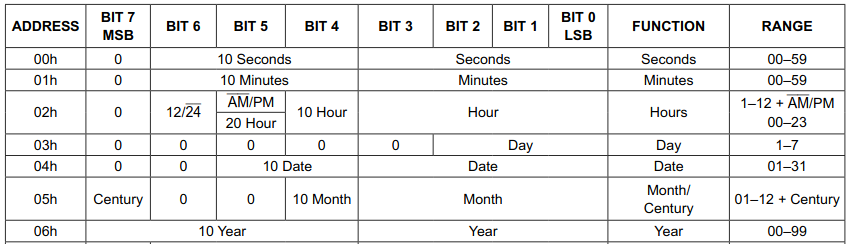
\includegraphics[width=0.8\textwidth]{images/timeDateRegisters}
	\caption{Time and Date Register Layout}
	\label{fig:images-timeDateRegisters}
\end{figure}

The code in Listing \ref{lst:writeTimeDate} shows the ``writeTime'' and
``writeDate'' functions, which pass the input character array values to the
``writeToReg'' function in order to be written to the RTC. As the upper nibble
of the ``Hours'' register contain control bits, these bits must not be modified
during a write operation. The ``hrRegChangeUpperBits'' function modifies only
the LSB of the upper nibble. The ``Dates'' register contains a ``10 Date''
value, to which a value is assigned using the ``dateChangeUpperBits'' function.
A check is used within the ``writeDate'' function to test if the date value is
within the appropriate range.

\lstinputlisting[language=C++, caption={writeTime and writeDate Functions}, label={lst:writeTimeDate}]
{snippets/writeTimeDate.cpp}
